\documentclass{../exercisesheet}

\title{Datenkommunikation und Informationssysteme, Übung 3}
\author{
    Domenic Quirl \\ 354437
    \and
    Julian Schakib \\ 353889
    \and 
    Daniel Schleiz \\ 356092
}

\renewcommand{\Exercise}{Aufgabe}
\date{Übungsgruppe 14}

\usepackage{float}
%\usepackage{siunitx}

\begin{document}
\maketitle
\pointtable

\begin{exercise}{1.5}
	\begin{subexercise}
	Da $10\text{W}=10000\text{mW}$ ergibt sich durch Einsetzen und Subtraktion der Dämpfung von $30 + 25 = 55\text{dB}$ eine Empfangsleistung von
	\[
		10 \cdot \log_{10}\left(\frac{10000\text{mW}}{1\text{mW}}\right) - 55 = 10 \cdot 4 - 55 = -15 \text{ [dBm]}
	\]
	\end{subexercise}
	
	\begin{subexercise}
	Die Dämpfung bestimmt maßgeblich die nutzbare Bandbreite eines Kommunikationskanals. Abhängig von der Frequenz variiert die Dämpfung. Unter bzw. ab
	einer gewissen Frequenz ist die Dämpfung so groß, dass Signale nicht mehr zuverlässig ausgewertet werden können. Es ergibt sich dadurch ein gewisser Bereich
	des Frequenzbands, abhängig vom Medium und dessen Eigenschaften, welcher effektiv benutzt werden kann, die nutzbare Bandbreite.
	\end{subexercise}
\end{exercise}

\begin{exercise}{3}
	\begin{subexercise}
	Da der Datenstrom 0110 halb so lang ist wie die Chipping-Sequenz, ergibt sich eine bit period von 2, d.h. es wird berechnet:
	\begin{table}[H]
	\centering
	\begin{tabular}{ll}
     	  & 00111100 \\
	$\oplus$ & 01110110 \\ \cline{2-2} 
     	 \rule{0pt}{3ex} & 01001010
	\end{tabular}
	\end{table}
	Somit wird 01001010 übertragen.
	\end{subexercise}

	\begin{subexercise}
	Zunächst ist der Multisensor 2000+ mit keinem der anderen Geräte kompatibel, denn er würde...
	\begin{itemize}
	\item ab 640ms für 64ms lang gleichzeitig mit dem Kohlenmonoxidsensor und dem Feuermelder senden.
	\item ab 448ms für 64ms lang gleichzeitig mit dem Bewegungsmelder senden
	\item ab 1408ms für 64 ms lang gleichzeitig mit dem Multisensor 2000+ v2 senden.
	\end{itemize}
	Da die Sendevorgänge periodisch auftauchen, werden sich diese Überschneidungen öfter wiederholen, und ist der Multisensor 2000+ in keiner Kombination
	mit anderen Geräten für einen Zeitmultiplex geeignet.\\
	Ansonsten überschneiden sich noch der Feuermelder und der Kohlenmonoxidsensor, z.B. bei 640ms für 64 ms lang und sind deshalb auch nicht kompatibel.\\
	Im Folgenden wird die Summe aus Sendelänge und Periode als \textit{Zyklus} bezeichnet. Die Kombinationen aus Bewegungsmelder und Feuermelder bzw.
	Bewegungsmelder und Kohlenmonoxidsensor weisen jeweils die gleiche Zykluslänge von 512ms auf. Betrachtet man nun jeweils für die beiden Kombinationen
	die ersten 512ms (beginnend bei 0), so sieht man am Versatz, dass es dort zu keinen Überschneidungen kommt, da der Bewegungsmelder 192ms nach dem
	Feuermelder sendet und der Kohlenmonoxidsensor 256ms vor Sendebeginn des Bewegungsmelders mit seiner Übertragung fertig ist. Aufgrund gleicher Zykluslänge
	kommt es also jeweils nie zu Überschneidungen.\\
	Außerdem sind die beiden gerade genannten Kombinationen jeweils mit dem Multisensor 2000+ v2 kompatibel, denn: dieser weist die doppelte Zykluslänge von
	1024ms, es genügt also den Zeitraum zwischen 0ms und 512 ms auf Kollisionen zu untersuchen, da der Multisensor 2000+ v2 im Vergleich zu den anderen
	beiden Kombinationen nur in jedem zweiten Zyklus von 512ms sendet. Es kommt ebenfalls zu keinen Kollisionen, da der Multisensor 2000+ v2 zwischen dem
	Feuermelder und Bewegungsmelder bzw. Kohlenmonoxidsensor und Bewegungsmelder sendet.\\ \ \\
	Mengen von kompatiblen Geräten wären somit \textbf{Feuermelder, Bewegungsmelder, Multisensor 2000+ v2} bzw. \textbf{Kohlenmonoxidsensor,	
	Bewegungsmelder, Multisensor 2000+ v2} und die jeweiligen Teilmengen. \\
	Daraus folgt, dass die maximale Anzahl an Geräten, welche gleichzeitig betrieben werden können, 3 beträgt. (Die beiden gerade erwähnten Kombinationen.)
	\end{subexercise}
\end{exercise}


\begin{exercise}{3}
	\begin{subexercise}
	Es kommt überall zu Problemen, wo die gewählte Rahmenbegrenzung in den Nutzdaten vorkommt, da in diesem Fall Nutzdaten als Steuerungszeichen aufgefasst werden und vom Empfänger als Rahmenbegrenzung interpretiert werden können. In den gegebenen Nutzdaten tritt dies an den unterstrichenen Stellen auf:
		1\underline{101 01}\ \underline{10 101}0 0101 001\underline{1 0101} 0011 1001
	\end{subexercise}

	\begin{subexercise}
	\begin{itemize}
	\item[(i)] 1101 \textbf{0}011 01\textbf{0}0 1001 01\textbf{0}0 0110 1\textbf{0}01 0011 1001
	\item[(ii)] 1\textbf{111 11}1\textbf{1 1111} 100\textbf{1 1111} 01\textbf{11 111}1 0011 1001
	\end{itemize}
	\end{subexercise}

	\begin{subexercise} 
		Strategie (i) stößt schnell an ihre Grenzen, sobald in den zu übertragenden Nutzdaten die Sequenz 1011 vorkommt. Diese würde dann zu 10101 ersetzt und das Flag wäre unerwünscht in den Daten enthalten.\\
		
		Auch Strategie (ii) kann einen solchen Fall verursachen, zum Beispiel bei der Übertragung von 1010 0101 1101, welches dann zu 11111 0101 1101 ersetzt würde. Dies sollte allerdings seltener auftreten als bei (i), da die Fehler verursachende Sequenz spezifischer ist. Beide Strategien verursachen bei einer Ersetzung dieselbe Verlängerung der Daten um 1 Bit, auch das sollte aber bei Strategie (ii) weniger häufig passieren, da die Sequenz, welche hier ersetzt wird, länger ist.\\
		
		Insgesamt ist also Strategie (ii) als weniger fehleranfällig und weniger zusätzliche Daten produzierend vorzuziehen.
	\end{subexercise}
\end{exercise}

\begin{exercise}{1}
	Ein Paket der Länge 40 Byte beinhaltet $40*8=320$ Bit und ist nur dann fehlerfrei, wenn alle Bits fehlerfrei sind. Die Wahrscheinlichkeit für ein Bit, fehlerfrei zu sein, ist $1-10^{-4}=0.9999$. Die Wahrscheinlichkeit, dass alle Bits fehlerfrei sind, ist demnach $0,9999^{320}\approx 0.96850503236$. Die Wahrscheinlichkeit für ein Paket, fehlerhaft zu sein, ist dementsprechend $1-0.96850503236\approx 0.03149496764\approx 3.1*10^{-2}$.
	
	Analog ergibt sich für ein Paket der Länge 1400 Byte $1400*8=11200$, $0.9999^{11200}\approx 0.32626152224$ und damit eine PER von $1-0.32626152224\approx 0.67373847776\approx
6.7*10^{-1}$.\\
\end{exercise}

\begin{exercise}{2.5}
	\begin{subexercise}
	Es ergibt sich
		\begin{equation*}
		\begin{split}
		&111010 \quad 0 \\
		&010011 \quad 1 \\
		&011101 \quad 0 \\
		&110111 \quad 1 \\
		&011001 \quad 1 \\[1em]
		&011010
		\end{split}
		\end{equation*}
	\end{subexercise}

	\begin{subexercise}
	\textbf{(i)}
	\begin{adjustwidth}{10pt}{10pt}
	Wähle die (verschiedenen) Bitfolgen 01101001 und 11101001. Mit Längsparität und den sonstigen Voraussetzungen werden diese kodiert zu
	0110\textbf{0}1001\textbf{0} und 1110\textbf{1}1001\textbf{0}, der Hamming-Abstand beträgt also 2. Dies ist hier minimal, denn: Unterscheiden sich
	zwei Bitfolgen nur um 1 Bit, so wird sich das Paritätsbit im entsprechenden Block ebenfalls unterscheiden. Unterscheiden sich nun 2 Bits zwischen den
	zwei Bitfolgen (im selben Block), so erhält man zwar das gleiche Paritätsbit, jedoch hat man bereits einen Hamming-Abstand von 2. Für mehr Bitflips
	oder zwei Bitflips in unterschiedlichen Blöcken hat man stets eine größere Hamming-Abstand, somit ist 2 minimal.
	\end{adjustwidth}
	\textbf{(ii)}
	\begin{adjustwidth}{10pt}{10pt}
	Wähle die (verschiedenen) Bitfolgen 01101001 und 11101001. Mit Kreuzparität ergeben sich: (durch Querparität entstandener Teil \textit{kursiv})\\
	0110\textbf{0}1001\textbf{0}\textit{1111} und 1110\textbf{1}1001\textbf{0}\textit{0111} und dadurch ein Hamming-Abstand von 3. Dies ist minimal,
	denn: Für einen Bitflip ergeben sich zwei geänderte Paritätsbits, einmal für die Längs- und einmal für die Querparität. Flippt man zwei Bits zwischen zwei
	Bitfolgen, so ist es optimal im Sinne des Hamming-Abstands, die zwei Bits innerhalb eines Blocks oder an der gleichen Position zwischen zwei Blöcken zu
	flippen. Dabei bleibt dann das Längs- oder Querparitätsbit gleich, jedoch ändern sich jeweils zwei Querbits bzw. zwei Längsbits. Somit erhäkt man einen Hamming-
	Abstand von 4. Man kann alle Änderungen an den Paritätsbits "aufheben", indem man einen "Viererblock" (Jeweils zwei Bits an der gleichen Position in
	verschiedenen Blöcken flippen), jedoch ist man dann schon Beim Hamming-Abstand 4. Somit ist der Hamming-Abstand 3 minimal.
	\end{adjustwidth}\ \\
	Insgesamt folgt, dass der minimale Abstand \textit{nicht} abhängig ist von der Blockgröße, da man in beiden Fällen durch einen Bitflip zwischen zwei
	Bitfolgen den minimalen Hamming-Abstand erreicht.
	\end{subexercise}
\end{exercise}

\begin{exercise}{4}
	\begin{subexercise}
	Da das Generatorpolynom Grad 4 hat, hänge an die Bitsequenz 01110101 die Bitfolge 0000 an und berechne den Rest bei Division mit 11001:
	\begin{figure}[h]
 		\centering
		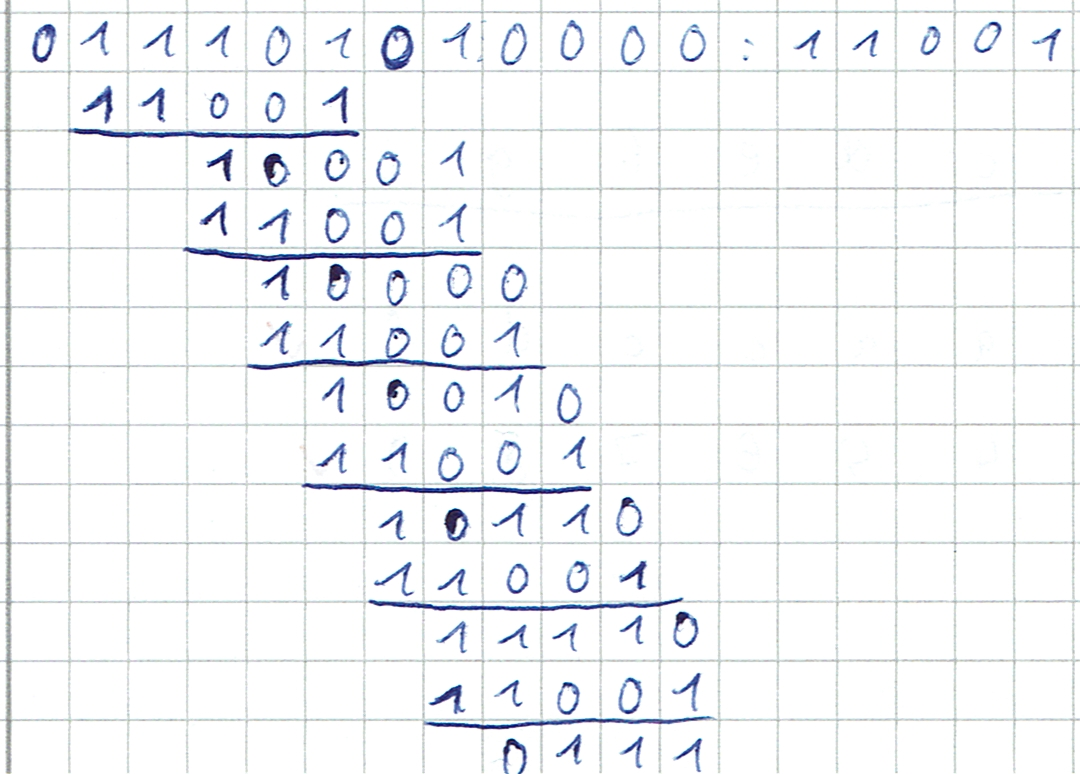
\includegraphics{3_6a.png}
	\end{figure}\ \\
	Die Prüfsumme entspricht dem Rest der Division, also 0111.
	\end{subexercise}
	
	\begin{subexercise}
	Berechne den Rest bei Division der empfangenen Bitsequenz mit der Bitfolge 11001 des Generatorpolynoms:
	\begin{figure}[h]
 		\centering
		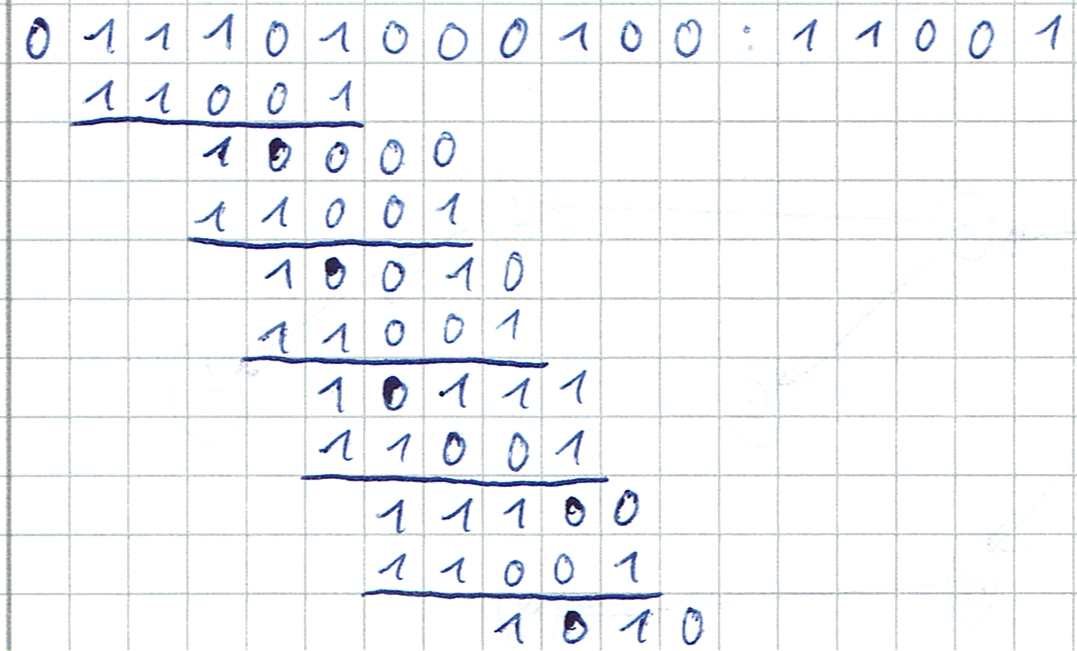
\includegraphics{3_6b.png}
	\end{figure}\ \\
	Da der Rest der Division ungleich 0000 ist, ist bei der Übertragung ein Fehler passiert.
	\end{subexercise}

	\begin{subexercise} 
	Die 3 gekippten Bits sind fett markiert: 011\textbf{01}10\textbf{0}0111. Der Fehler wird nicht erkannt, da die Division mit dem Generatorpolynom
	den Rest 0 lässt:
	\begin{figure}[h]
 		\centering
		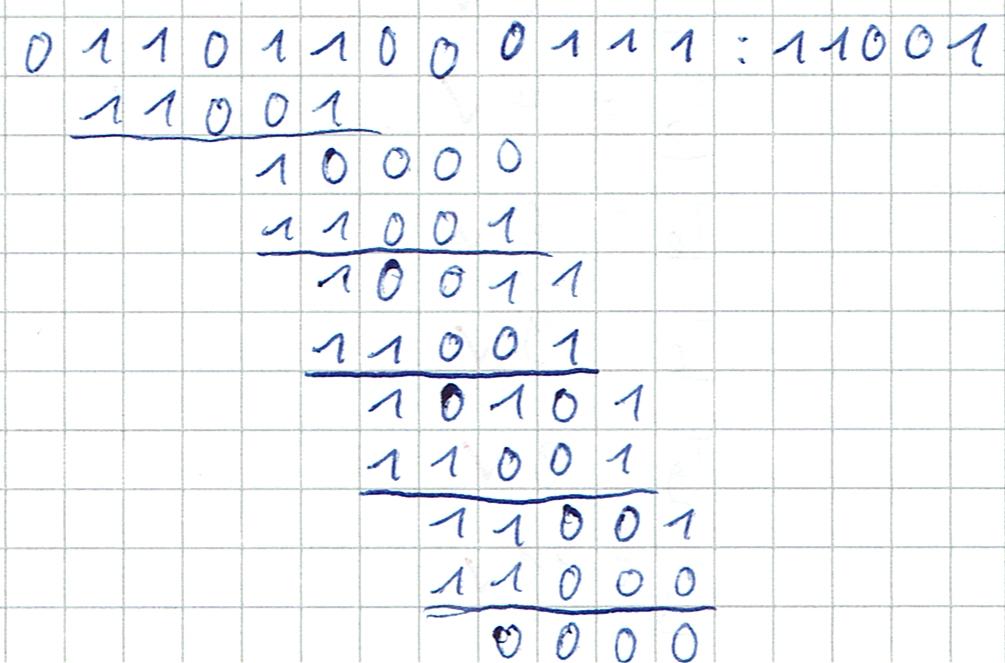
\includegraphics{3_6c.png}
	\end{figure}
	\end{subexercise}
\end{exercise}

\end{document}
